%----------------------------------------
% SECTION: Quantum simulation
%----------------------------------------
\section{Quantum simulation}
\label{sec:quantum_simulation}

Simulating quantum mechanics is a very challenging task, especially if one is interested in many-body systems.
The description of a state requires a large number of parameters, for keeping track of all the quantum amplitudes, and it grows exponentially with the system size.
Hence, one would have an \emph{exponential explosion} in terms of \emph{classical} resources (e.g., computer memory), which clearly is not suitable.
If simulating a quantum system is not a task for classical computers, then it is reasonable to assume that it might be a task for \emph{quantum computers}.
This kind of devices, first envisioned from Feynman \cite{feynman2018simulating}, promises much more than simulating quantum mechanics.
Indeed, quantum computation and quantum information theory are, still today, very active research fields \todo{inserire reviews}\citneeded.

Using quantum mechanics for simulating quantum mechanics may seem like fighting fire with fire, but it is a totally reasonable approach.
A quantum computer can encodes the large amount of information of a quantum system in its large number of amplitudes.
So, the size of a quantum computer would only be proportional to the size of the quantum system it intends to simulate, \emph{without} an exponential explosion in \emph{quantum} resources.
In fact, a quantum computer can indeed act as a \emph{universal quantum simulator} \cite{lloyd1996simulator}.
This is basically the idea behind \emph{digital \acl{qs}}.

There is another kind of approach to quantum simulation, where one can mimic the evolution of a given quantum system by means of another \emph{analogous} and \emph{controllable} quantum system.
Hence, we will only need a specific quantum machine for a specific class of problems and a full general-purpose quantum computer is not needed.
% In this case, for a specific set of problems the full implementation of a quantum computer may not be necessary.
This is the idea behind \emph{analog \acl{qs}}.

In general, \emph{\acf{qs}} can be (loosely) defined as simulating a quantum system by quantum mechanical means.
There are three paths that can be taken in this regard:
\begin{itemize}
    \item Digital \acl{qs}
    \item Analog \acl{qs}
    \item Quantum Information inspired algorithms for classical simulation
\end{itemize}
We will discuss briefly each one of them.
By \emph{quantum simulator} we mean a \emph{controllable} quantum system used to simulate or emulate other quantum systems.
We see that only digital and analog \ac{qs}s employ a quantum simulator.
The last option employs techniques, inspired by quantum information theory, that make it possible to truncate and approximates quantum states in order to have efficient classical simulations.


\begin{figure}[t]
    \centering
    \begin{tikzpicture}[
    ket/.style = {font=\Large},
    ->/.style={-stealth, ultra thick, shorten >=3pt, shorten <=3pt, Grey60},
    system/.style = {draw, dotted, thick, rounded corners, inner sep=10pt},
    simulator/.style = {draw, thick, rounded corners, inner sep=10pt}
    ]
    \node[ket] (phi0) at (0, 2.5) {$\ket{\phi(0)}$};
    \node[ket] (phit) at (3, 2.5) {$\ket{\phi(t)}$};
    \node[ket] (psi0) at (0, 0) {$\ket{\psi(0)}$};
    \node[ket] (psit) at (3, 0) {$\ket{\psi(t)}$};

    \begin{scope}[on background layer]
        \node[fit=(phi0) (phit), system, label=above:{Quantum System}, fill=Blue, fill opacity=0.1] {};
        \node[fit=(psi0) (psit), simulator, label=above:{Simulator}, fill=Blue, fill opacity=0.1] {};
    \end{scope}

    \path (phi0) edge[->] node[above, black] {$U$} (phit);
    \path (psi0) edge[->] node[above, black] {$U^{\prime}$} (psit);

    \path (phi0) edge[->, dashed] (psi0);
    \path (psit) edge[->, dashed] (phit);

    \node (prep) at (0, -1.5) {preparation};
    \node (meas) at (3, -1.5) {measurement};

    \path (prep) edge[->] (psi0);
    \path (psit) edge[->] (meas);
\end{tikzpicture}

    \caption{Schematic picture of a quantum simulator.}
\end{figure}



\subsection{Digital quantum simulations}
\label{sub:digital_quantum_simulations}

The digital approach to \ac{qs} employs the \emph{circuit model} of quantum computation.
This model is analogous to the boolean logic model of classical computation, where one works with \emph{bits}, the smallest possible amount of information, an on--\emph{or}--off state, and \emph{logical operators} (like \texttt{NOT}, \texttt{AND}, \texttt{OR}, etc\dots).
The quantum counterpart uses \emph{qubits}, the smallest possible quantum system which is a two-level system, and \emph{unitary operators}, also called \emph{quantum gates}.
The set of qubits forms a \emph{quantum register} and it is where the information about the simulated system is encoded.
% Generally, the quantum simulator is a collection of \emph{qubits} (i.e., two-level quantum systems) called a \emph{quantum register}.
% This register is then used to simulate the wave function of the target quantum system.
In the \emph{computation basis}, the wave function of the register is in a superposition of bit strings, where each bit refers to the state of a qubit in the register, which can be either $\ket{0}$ or $\ket{1}$.

In the circuit model, any many-qubit unitary operator $U$ can be converted into a sequence of single- and two-qubit quantum gates.
Therefore, any generic unitary evolution can be implemented with a minimal set of quantum gates\citneeded.
This minimal set is usually composed of a number of single-qubit gates (for example, the Hadamard gate or the Pauli matrices) and a two-qubit \emph{entangling gate}, like a \texttt{CNOT} gate.
% An example of a relevant unitary operator is the time-evolution operator, that solves the time-independent Schrödinger equation.
Even though it has been proven \cite{lloyd1996simulator} that ``anything'' can be simulated on a quantum computer, not all unitary operations can be simulated \emph{efficiently}.
Therefore, there are \emph{mathematically possible} Hamiltonians that cannot be efficiently simulated with a circuit-based model.
Nonetheless, it is believed that \emph{physically relevant} Hamiltonians can indeed be simulated efficiently\citneeded.

It should be stressed that we are still far from perfect digital quantum computation.
A number of problems afflict quantum computers to this day.
The first one is error correction and error detection.
As one would expect, a quantum register is very delicate object and the presence of noise could, at any time, flip any of the qubits or modify the relative phases, which will spoil the encoded information.
Another problem comes from \emph{decoherence}, where the interaction with the environment induces a \emph{loss of information}.



It should be stressed that the implemented unitary operations are often just approximations of the desired unitary operation.
With greater precision comes a greater number of gates.

The typical setup for a digital simulation consists of three steps:
\begin{description}
    \item[Initial-state preparation] the quantum register has to prepared in the initial state $\ket{\psi(0)}$.
        This step can be by itself difficult, and it is not always guaranteed that an efficient algorithm may exist.

    \item[Unitary evolution]  the circuit has to reproduce or simulate the action of a unitary operator $U$.
        In case of a unitary time evolution and local Hamiltonian this can be achieved approximately with some ``trotterization'' scheme.

    \item[Final measurement] after obtaining the wanted state $\ket{\psi(t)} = U \ket{\psi(0)}$, a \emph{measurement} is needed in order to extract relevant physical information.
        Instead of capturing the whole wave function $\ket{\psi(t)}$, with, for example, quantum tomography, one may proceed with the direct estimation of certain physical quantities, such as correlation functions or spectra of operators.
\end{description}


\todo{cosa altro aggiungere?}

\begin{figure}[t]
    \centering
    \newcommand{\Gate}[3]{\draw[gate] (#1, -#2 + 0.25) rectangle ++(1.5, -#3 - 0.5);}
    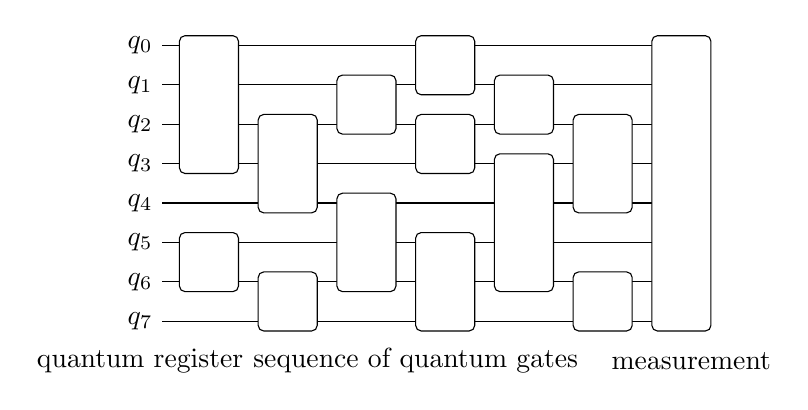
\begin{tikzpicture}[
        scale=0.5,
        gate/.style = {rounded corners=2pt, fill=white}
        ]
        \foreach \n in {0,...,7} {
            \node (q\n) at (0, -\n) {$q_{\n}$};
            \node (q\n end) at (14, -\n) {};
            \path (q\n) edge (q\n end);
        }
        % \draw[gate] (1, 0 + 0.25) rectangle ++(1.5, -3 - 0.5);
        \Gate{1}{0}{3}
        \Gate{1}{5}{1}
        \Gate{3}{2}{2}
        \Gate{3}{6}{1}
        \Gate{5}{1}{1}
        \Gate{5}{4}{2}
        \Gate{7}{5}{2}
        \Gate{7}{2}{1}
        \Gate{7}{0}{1}
        \Gate{9}{3}{3}
        \Gate{9}{1}{1}
        \Gate{11}{2}{2}
        \Gate{11}{6}{1}
        \Gate{13}{0}{7}

        \node at (0, -8) {quantum register};
        \node at (7, -8) {sequence of quantum gates};
        \node at (14, -8) {measurement};
    \end{tikzpicture}
    \caption{Example of a quantum circuit \todo{da finire}.}
\end{figure}


\subsection{Analog quantum simulations}
\label{sub:analog_quantum_simulations}

Analog \ac{qs} (AQS) represent another kind of approach to \ac{qs}, where a one quantum system mimics or emulate another.
The Hamiltonian of the system to be simulated, $H_{\text{sys}}$, is directly mapped onto the Hamiltonian of the quantum simulator, $H_{\text{sim}}$.
Obviously, this can be done if there is a mapping between the system and the simulator.
Note that the simulator may only partly reproduce the dynamics of the system, or simulate some effective description of the system.

An important advantage of analog \ac{qs} is that it does not require a full quantum computer.
Even more, the simulator does not even need to be a computer at all.
Finding the mapping in an analog \ac{qs} might look, at first, simpler than finding the most efficient gate decomposition of a Hamiltonian, but it is not always true and there are no recipes ready for constructing these mappings in a general case.
The obvious drawback of AQS is that the quantum simulators are problem specific, but on the other hand, given that they do not require a full quantum computer, they are more feasible in the near-term.


\todo{Aggiungere altro ma cosa?}


\subsection{Quantum-inspired algorithms}
\label{sub:quantum_inspired_algorithms}

Thanks to the developing science of quantum information, new \emph{classical algorithms} have been invented for the simulation of quantum many-body systems.
One of the most important examples of these quantum-inspired algorithms are \emph{tensor networks} methods\todo{inserire citazioni di review}\citneeded.

Tensor networks make it possible to ``compress'' the information about a many-body wave function by expressing it as a contraction of a network of tensors (as suggested by the name).
In details, to each physical site we associate a tensor with a number of indices (or legs).
One of these indices is called the \emph{physical index} of the tensors, which runs over the basis of the local Hilbert space.
The other indices are \emph{auxiliary indices}, their dimension is governed by a parameter $\chi$ called the \emph{bond dimension} and are ``connected'' to other sites.
Roughly speaking, these auxiliary indices encodes the entanglement information between the connected sites.

For a large class of physically relevant models, the ground state is gapped and has, in a certain sense, a finite amount of entanglement.
This fact is expressed by the so-called \emph{area law}, where the entanglement between two partitions of the system grows with size of the boundary, the area between the two partitions, and not with the size of the partition itself.
The main advantage of tensor networks is their ability to capture this area law.

\todo{Aggiungere altro}
